
\begin{center}
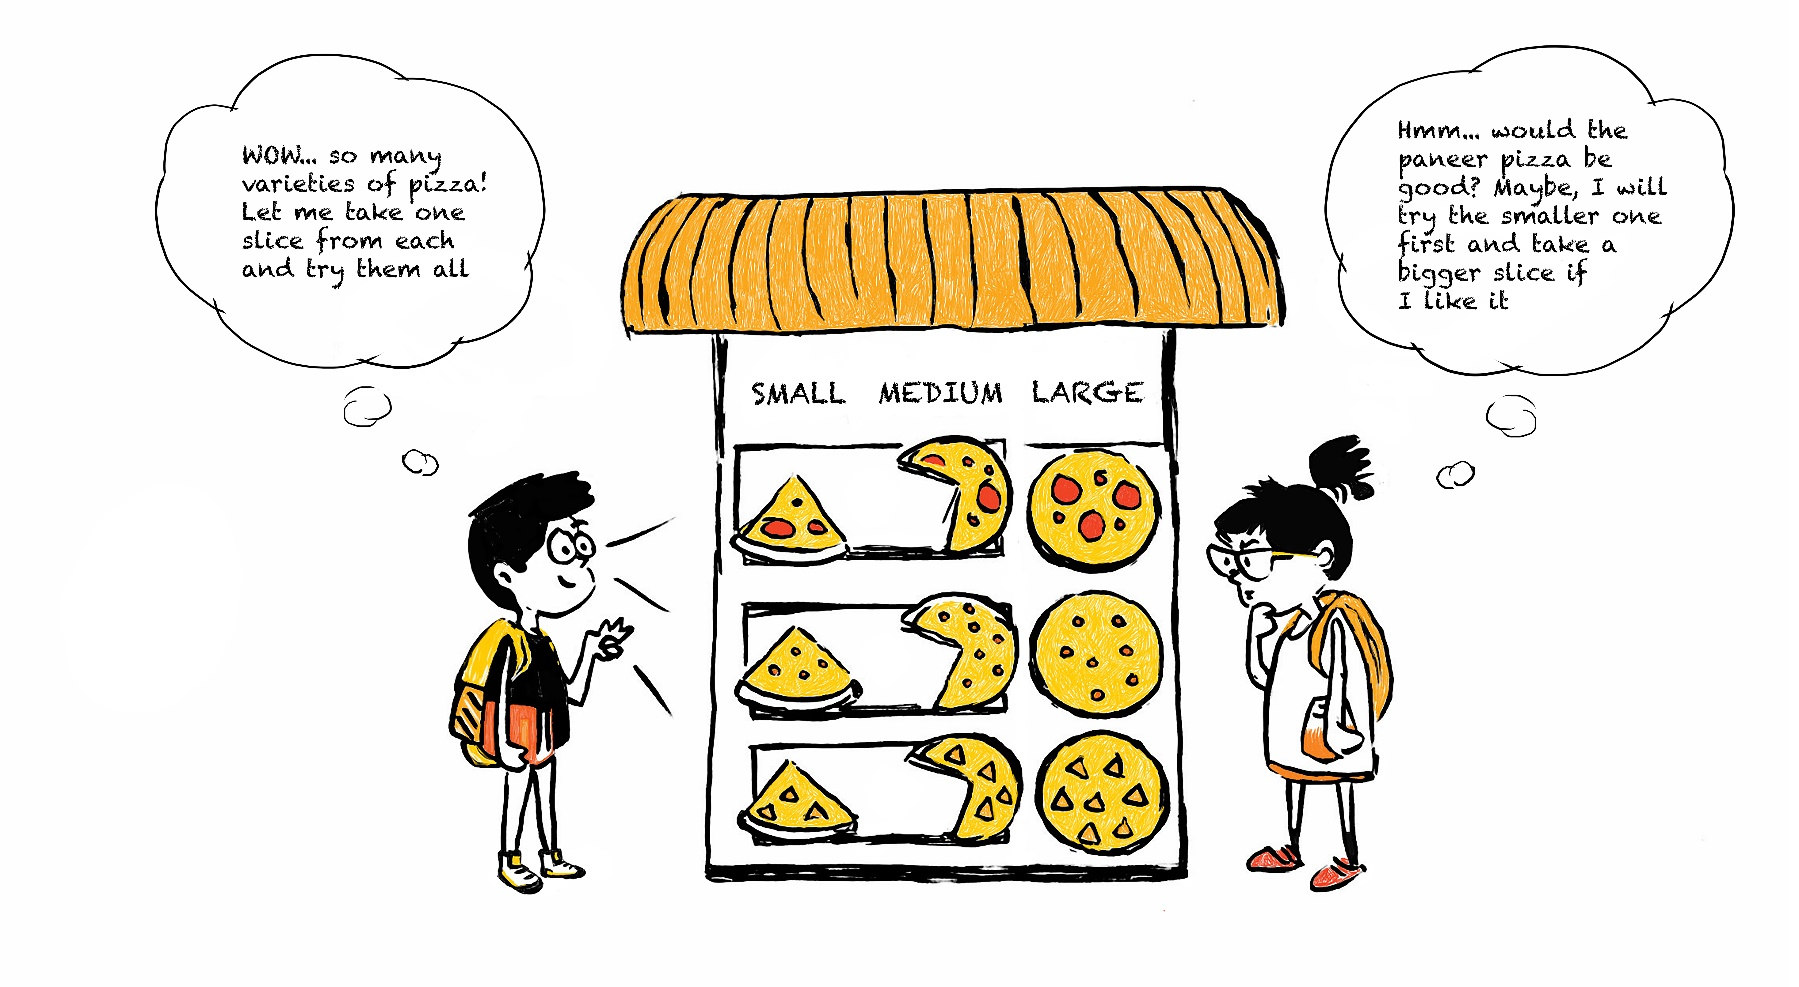
\includegraphics[height=7cm]{./parts/fractal-pizza}
\end{center}

\section{GLOSSARY OF TERMS }
\begin{itemize}
\item {\bf Credit:} The quantitative measure of recognition given to a course, stated in semester hours. Typically, a theory course running for a full a semester with three contact hours per week would be 3 credits. Similarly, a lab course with the same number of contact hours would be 2 credits.  
\item {\bf Major:} The primary set of discipline-specific coursework pertaining to the student’s department/discipline  
\item {\bf Minor:} Additional basket of coursework done from a discipline different from the student’s original discipline (and would also find mention in the final degree)
Honors: Additional basket of coursework done in the same discipline as the student’s original discipline (and would also find mention in the final degree)
\item {\bf Double Major:} Coursework pertaining to two departments/disciplines and leading to two separate degrees.
\item {\bf Additional Course:} An additional course taken by the student over and above the minimum credit requirements of the degree. 
Pre-requisite: The preliminary requirement, usually successful completion of another course, that must be met before a course can be taken.
\item {\bf Elective:} Course chosen by the student and which would form part of his/her degree requirements. 
\item {\bf Free Elective:} A course of the student’s choice, to be selected from the any department (subject to meeting the pre-requisites) 
\item {\bf Core Elective:} A course of the student’s choice, to be selected from the same department (or offered by a different department, but identified as "core" by one's department)
\item {\bf LA/CA Elective:} A course of the student’s choice, to be selected from the Liberal Arts and Creative Arts category 
\item {\bf Science Elective:} A course of the student’s choice, to be selected from the Maths, Physics \& Chemistry list of courses
\item {\bf Fractal Segment:} The part or duration of a semester in which a particular course is offered
\end{itemize}

\section{COURSE NUMBERING SCHEME}
Each course is denoted by a course number consisting of two letters followed by four numerals.
\begin{center}
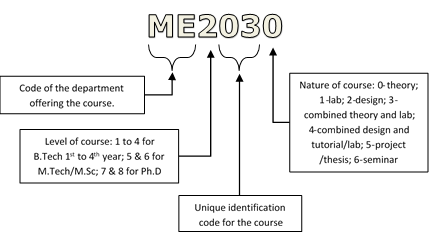
\includegraphics[height=4.5cm]{./parts/course-code}
\end{center}


\section{FRACTAL SEGMENTS}
In the fractal system, a semester is divided into six segments. Each segment is approximately 2.5 to 3 weeks in duration. Every fractal course is accompanied by a two-digit segment number indicating the duration of the course. The first number denotes the segment in which a course will begin and the second number the segment in which it will be completed. For example, Segment 34 means, a particular course will begin in segment-3 and finish at the end of segment-4. Typically, a course running for full the semester (i.e., all six segments) would be 3-credits; so each segment will be equivalent to 0.5 credit. Accordingly, the credit of a course will be decided, based on its segment data. For example, if the segment of a course is 56, it implies that the course will be running in two segments (5 \& 6). Hence, it will be $0.5 \times 2 = 1$ credit. 

\begin{center}
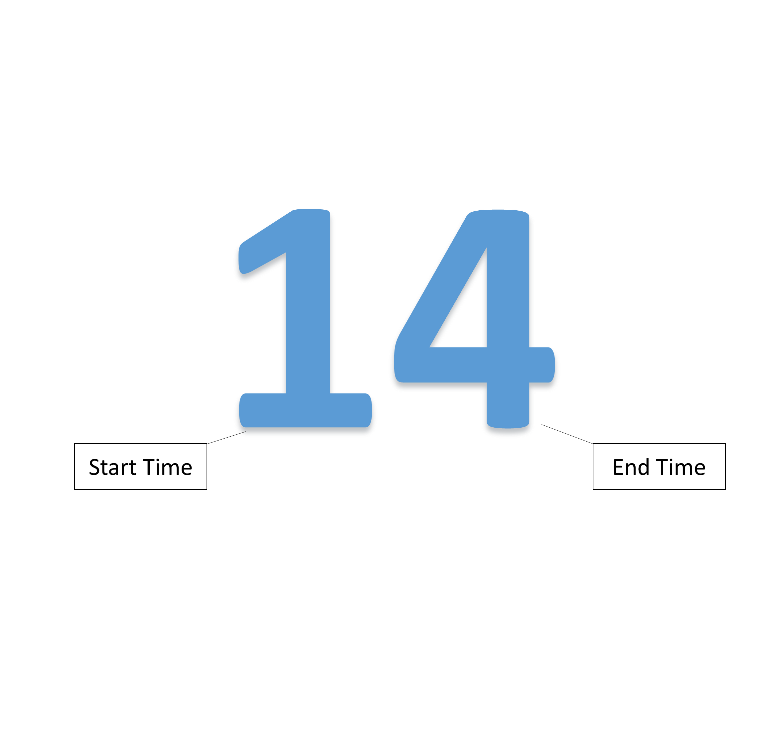
\includegraphics[height=2cm]{./parts/course-segment}
\end{center}

\begin{tabular}{|c|c|c|c|c|c|c|}
    \hline
    & \multicolumn{6}{|c|}{SEMESTER} \\ \hline
    SEG CREDITS & 1 & 2 & 3 & 4 & 5 & 6 \\ \hline
    0.5 & \multicolumn{1}{|c|}{11}& \multicolumn{1}{|c|}{22}& \multicolumn{1}{|c|}{33}& \multicolumn{1}{|c|}{44}& \multicolumn{1}{|c|}{55}& \multicolumn{1}{|c|}{66} \\ \hline
    1.0 &\multicolumn{2}{|c|}{12}& \multicolumn{2}{|c|}{34} & \multicolumn{2}{|c|}{56} \\ \hline
    1.5 &\multicolumn{3}{|c|}{13}& \multicolumn{3}{|c|}{46} \\ \hline
    2.0 &\multicolumn{4}{|c|}{14}& \hspace{2mm} & \hspace{2mm}  \\ \hline
    2.0 & \hspace{2mm} & \hspace{2mm} & \multicolumn{4}{|c|}{36} \\ \hline
    3.0 &\multicolumn{6}{|c|}{16} \\ \hline
\end{tabular}
